\section{EXPERIMENTS AND EVALUATION}
\label{sec:exper}

\begin{figure}[t]
	\centering
	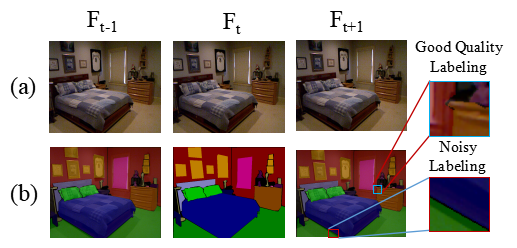
\includegraphics[scale=0.48]{figure/PGT.png}
	%	\vspace*{-0.6cm} 
	\caption{Propagated pseudo ground truth from a reference frame $F_t$ to $F_{t+1}$.\comments{The GT of $F_t$ is provided by NYU-v2 dataset. We propogate the annotated label of $F_{t}$ to $F_{t+1}$ and generate the corresponding PGT.} Most of the pseudo labels are reliable, while there are some noisy around object boundaries.}
	\label{fig:PGT}
	%	\vspace*{-0.35cm} 
\end{figure}

\begin{figure}[!th]
	\centering
	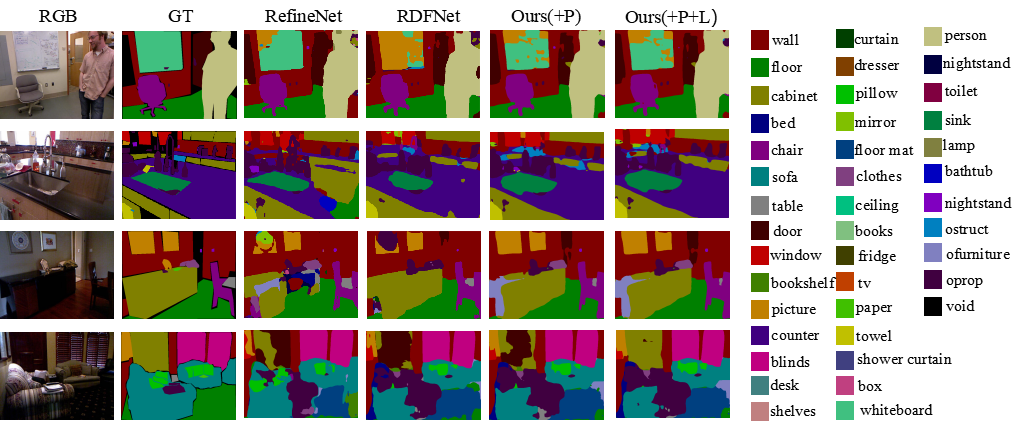
\includegraphics[scale=0.42]{figure/Result.png}
	\caption{Qualitative results on the NYUD—v2 dataset. For the secne image in each row, we show: the input image; the ground truth of semantic segmentation; the result of RDFNet; The result of our method. Our method predicts more accurate segmentation result.}
	\label{fig:VisResult}
\end{figure}

In order to evaluate the proposed method for indoor scene segmentation, we conduct experiments on a publicly available benchmark dataset (NYUD-v2) and show the superiority of our method.
%, which contains 273 video sequences of RGBD data.  


\noindent\textbf{Dataset.}  
The NYUD-v2 dataset constains in total 464 RGB-D video sequences of indoor scenes. 
%
For the task of semantic segmentation, 1449 images are manually annotated, among which 795 images are used for training and the remaining 654 images for testing.
%
In our experiment, we map the semantic labels into 40 categories, similar as \cite{Gupta2014}.
%
From the 795 manually labeled images for training, we propagated these GT labels to 14344 unlabeled frames, and filtered out 5897 frames by homography matrices, and filtered out 821 frames by manual check. 
We finally obtained 7626 frames with pseudo ground truth. 
%
Comparing with dense image annotation, filtering PGT for 273 videos took about 8 hours for a graduate student.
%
Although the generated pseudo labels still have a certain amount of noise, the diversity of training set is greatly enriched. 



The training images, including both manually labeled images and propagated images, are augmented by random horizontal flips with a possibility of 0.5, scaling with a randomly selected ratio in $\left\{0.7,0.8,0.9,1.0,1.2,1.3\right\}$ and random cropping. 
%
All our experiments are conducted on a single Nvidia Titan X Pascal GPU, using the Caffe framework.

\noindent\textbf{Evaluation Metrics.}  
Following previous work
\cite{Eigen2015,Gupta2014,Kendall2015,Lin2016,Lin2017,Li2016,Cheng2017,Park2017,Xu2018,Zhang2018,Jiao2018}, we use three quantitative metrics to evaluate our semantic segmentation results, including pixel accuracy, mean accuracy and mean IOU. 
%%
Denote $m_{kj}$ as the number of pixels of class ${k}$ classified as class ${j}$
%Assuming 
The number of categories is $c$, and $M_{k} = \sum_{j}m_{kj}$ is the total number of pixels belonging to class $k$. 
%
And $N = \sum_{k}m_{k}$ denotes the number of all pixels in the training set.
%
The three metrics are defined as follows:
\begin{equation}\label{eq:metric}
\begin{array}{rl}
\text{pixel accuray}: &  \frac{1}{N}\sum_{k}m_{kk}, \\
\text{mean accuracy}: &\frac{1}{c}\sum_{k}\frac{m_{kk}}{M_{k}}, \\
\text{mean IoU}: &\frac{1}{c}\sum_{k}\frac{m_{kk}}{ M_{k}+\sum_{j}m_{jk}-m_{kk}}.
\end{array}
\end{equation}

%\renewcommand{\baselinestretch}{1.0}\indent\text{---} pixel accuracy: $\sum_{k}m_{kk}/I$;\\
%\indent\text{---} mean accuracy: $\frac{1}{c}\sum_{k}m_{kk}/m_{k}$;\\
%\indent\text{---} mean IOU: $\frac{1}{c}\sum_{k}m_{kk}/(m_{k}+\sum_{j}m_{jk}-m_{kk})$ ;\\




\begin{table}[tb]
%	\vspace{-0.4cm}
	\centering
	\caption{Comparison of different methods.}
	\begin{tabular*}{8.7cm}{llccc}
		\hline
		Method & Data & Pixel & Mean  & IoU\\
		       &     & accuracy & accuray  & \\
		\hline 
		B-SegNet \cite{Kendall2015} & RGB &68.0 & 45.8 & 32.4 \\
		Context \cite{Lin2016} & RGB & 70.0 & 53.6 & 40.6 \\
		RefineNet \cite{Lin2017} & RGB & 73.6 & 58.9 & 46.5\\
		\hline
		Gupta et al. \cite{Gupta2014} & RGBD & -- & 35.1 &--\\
		Eigen et al. \cite{Eigen2015} & RGBD & 65.6 & 45.1 & 34.1\\
		FCN \cite{Long2015} & RGBD & 65.4 & 46.1 & 34.0 \\
		LSTM-CF \cite{Li2016} & RGBD & --& 49.4 & -- \\
		Cheng et al.\cite{Cheng2017} & RGBD & 71.9 & 60.7 & 45.9 \\
		RDFNet \cite{Park2017} & RGBD & \bf{76.0} & 62.8 & 50.1\\	
		%\hline
		Baseline &RGBD & 75.8 & 63.0 & 50.0\\
		Ours (+$L_{C}$) & RGBD & 75.8 & 63.3 & 50.1\\
		Ours (+$PGT$) & RGBD & 75.9 & 63.6 & 50.2\\
		Ours (+$L_{C}$+$PGT$)& RGBD & 75.8 & \bf{63.8} & \bf{50.2}\\
		\hline
		PAD-Net \cite{Xu2018} & RGB &75.2 & 62.3 & 50.2\\
		TRL \cite{Zhang2018} & RGB &76.2 & 56.3 & 46.4\\
		Jiao et al.\cite{Jiao2018} & RGB & \emph{81.1} & 62.2 & \emph{50.9}\\
		\hline		 		
	\end{tabular*}
	\label{Tab:Results}
\end{table}



We set the RDFNet~\cite{Park2017} as our baseline. 
However, due to hardware difference, using the official code, we get results (Baseline) that is slightly different from that reported in their paper (RDFNet), as shown in Table~\ref{Tab:Results}. 
We compare different variant of our approach to demonstrate the effectiveness of each component, and the results are reported in Table~\ref{Tab:Results}. 

\para{Analysis of Temporal Consistency.} While training RDFNet with the 795 manually labeled images, and our temporal consistency constraint (+$L_C$ for short), the mean accuracy increases to $63.3\%$ from $63.0\%$, and IoU increases to $50.1\%$ from $50.0\%$.


\para{Analysis of Pseudo labels.} 
Though the pseudo labels still contains a certain amount of noises, most of them are reliable, especially inside an object region. 
%
While training the RDFNet with extra images of pseudo labels, the performance (Ours+PGT) greatly increases, especially at mean accuracy ($63.6\%$), compared with the baseline.
%
To facilitate future study, we will release our dataset with pseudo labels.
%

Combining both the pseudo ground truth and temporal consistency, our approach outperforms existing semantic segmentation networks, especially at mean accuracy and IoU metrics. 
We also compare our method with three multi-task learning techniques and our method achieves comparable performance.
%
Though Jiao et al achieve the best performance on pixel accuracy and IoU, they require additional dense ground-truth for depth estimation and much heavier computational cost.
%
Fig.~\ref{fig:VisResult} shows a group of segmentation results. It can be seen that our method performs well on objects such as pictures, whiteboards and so on. 
%

\comments{
\para{Analysis of Temporal Consistency.}  
To discover the effectiveness of our proposed training policy. 
%
We conduct our experiments on generated PGT data with temporal consistency loss.
%
The quantitative and qualitative results are shown in Table~\ref{Tab:Results} and
Fig.~\ref{fig:VisResult} respectively.
%
To prove that performance improvements are not just due to PGT, we did an ablation study by removing ${PGT}$.
%
The results are shown in Table~\ref{Tab:Results} and Fig.~\ref{fig:VisResult}.
%
Compared to baseline, the mean accuracy and IOU are all been promoted.
%
Using $L_{consistency}$ and $L_{PGT}$ simultaneously, the mean accuracy is improved by 0.8\%.
%
And mean IoU is improved by 0.2\%.
%
And our method achieves the comparable performance as multi-task learning method.
}


\para{Dicussion.} By involving temporal consistency, we also found that there are conflicts between manual labels of the same scene, as shown in Fig.~\ref{fig:mislabels}. Our method produce much more accurate and consistent results.
% the ground truth proposed by NYUD-v2 data set exits some annotation errors shown in Fig.~\ref{fig:mislabels}.


\begin{figure}[!htbp]
	\setlength{\abovecaptionskip}{-0.2cm}
	\setlength{\belowcaptionskip}{-10cm}
	\centering
	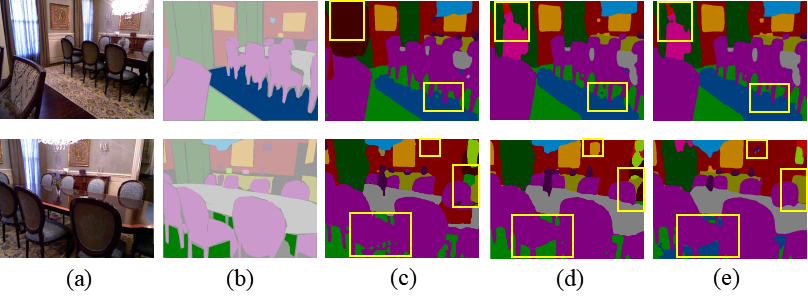
\includegraphics[scale=0.4]{figure/Mislabels.png}
	\caption{Mislabeled images. (a) Two frames of the same scene. (b) Their corresponding ground truth labels. Note the difference between the labels of the floor pixels. Blue as ``floor mat" and green as ``floor".  The mislabled pixels are highlighted. (c)(d)(e) The prediction results of RefineNet, RDFNet and our method, respectively.}
	\label{fig:mislabels}
\end{figure}
%

\comments{
But our proposed method shows a more robust result compared to RefineNet \cite{Lin2017} and RDFNet \cite{Park2017}.
%
There are still some difficult classes in NYUD-v2 data set, such as bag and box.
%
The pixel accuracy and IOU is under 30\%.
%
The main reason is that the size of these two kinds of object is too small and the occurrence frequency of them is very low. 
}





